%%This is a very basic article template.
%%There is just one section and two subsections.
%\documentclass{article}
\documentclass[preprint,12pt]{elsarticle}
\journal{Jornal Name in the document\ldots\ldots\ldots.}
\begin{document}



\begin{frontmatter}



\title {Face recgontion using Particle Swarm clustering  }


\author[label]{Maha El Meseery}
\author[label]{Mahmoud fakhr el Deen}
\author[label]{Heba Nemer}

\address[label1]{Electronic Research Institute, Cairo, Egypt}

\begin{abstract}
%% Text of abstract
The abstract of paper\ldots\ldots\ldots\ldots.

\end{abstract}

\begin{keyword}
My first keyword \sep keyworbd\ldots

\end{keyword}

\end{frontmatter}




\section{Introduction}

\section{Background Information}
\subsection{Particle Swarm Optimization}
%\section{Discrete Particle Swarm Optimization}
\label{sec:ParticleSwarmAlgorithm}
 The main idea of \textit{Particle Swarm Algorithm (PSO)} is to represent each solution with a $N$ dimension particle from the solution space \cite{PSOFirst}. Each particle moves with a direction and velocity $v_{ij}$ based on equations \ref{eq:Swarm1} \& \ref{eq:Swarm}.

\begin{equation}
%\[
p_{ij}=p_{ij}+v_{ij},
%\
\label{eq:Swarm1}
\end{equation}

where $p_{ij}$ represent the $j$th dimension in the $i$th particle and $v_{ij}$ is the velocity of the $j$th dimension in the $i$th particle.
 %Equation [\ref{eq:Swarm}] shows how velocity and direction of each particle are computed
 \begin{equation}
v_{ij}  = v_{ij} \omega + c_1 r_1 (lbest_{ij}  - p_{ij} ) + c_2 r_2 (gbest_{ij}  - p_{ij} ),
\label{eq:Swarm}
\end{equation}
 where $\omega$ is the inertia weight parameter which controls the tradeoff between exploration and exploitation,  $lbest_{ij}$ is the local best particle, $gbest_{ij}$ is the global best particle, $r_1$ \& $r_2$ are random variables and $c_1$ \& $c_2$ are the swarm acceleration parameters.

 After each iteration the global best $g_{best}$ particle and the agent local best particle $l_{best}$are evaluated based on the maximum fitness functions of all particles in the solution space. The solution is found after achieving a specific number of iteration or after an error threshold is achieved.
Equation \ref{eq:descrite} is used to change the general swarm algorithm into binary particle (\textit{Discrete Particle Swarm Algorithm DPSO}). The \textit{DPSO} handles particle values of either $0$ or $1$ \cite{PSODisceret}.
\begin{equation}
   P(i)\Leftarrow
\left \{
\begin{array}{c}
1 \quad \quad if\quad r_{3}>p_{i}  \\

0 \quad \quad if\quad r_{3}<p_{i},
\label{eq:descrite}
\end{array}\right.
\end{equation}
 where $p_{ij}$ is the numerical values of the particle and $r_{3}$ is a random variable.
\subsection{Eigen Faces}
\label{facereg}
A set of eigenfaces \cite{facesite} can be generated by performing a mathematical process called principal component analysis (PCA) on a large set of images depicting different human faces. Informally, eigenfaces can be considered a set of "standardized face ingredients", derived from statistical analysis of many pictures of faces. Any human face can be considered to be a combination of these standard faces.


 The aim is to represent a face as a linear combination of a set of basis images called eigenfaces. That is :
\begin{equation}
% MathType!MTEF!2!1!+-
% feaafiart1ev1aaatCvAUfeBSjuyZL2yd9gzLbvyNv2CaerbuLwBLn
% hiov2DGi1BTfMBaeXatLxBI9gBaerbd9wDYLwzYbItLDharqqtubsr
% 4rNCHbGeaGqiVu0Je9sqqrpepC0xbbL8F4rqqrFfpeea0xe9Lq-Jc9
% vqaqpepm0xbba9pwe9Q8fs0-yqaqpepae9pg0FirpepeKkFr0xfr-x
% fr-xb9adbaqaaeGaciGaaiaabeqaamaabaabaaGcbaGaeuOPdy0aaS
% baaSqaaiaadMgaaeqaaOGaeyypa0ZaaabCaeaacqaHjpWDdaWgaaWc
% baGaamyAaaqabaGccaWG1bWaaSbaaSqaaiaadQgaaeqaaaqaaiaadQ
% gacqGH9aqpcaaIXaaabaGaam4saaqdcqGHris5aaaa!444E!
\Phi _i  = \sum\limits_{j = 1}^K {\omega _i u_j }
\end{equation}

Where $\Phi_i$ represents the $i^{th}$ face with the mean subtracted from it, $\omega _i$ represent weights and  $u_j$ the eigenvectors.

This can be represented aptly in a figure as:

\begin{figure}[h]
 \begin{center}
 \centering
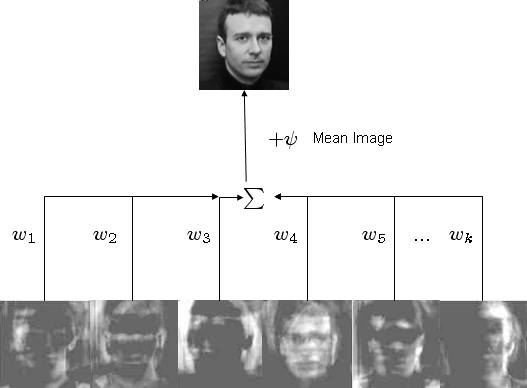
\includegraphics[scale=0.5]{eigenfacesrec.jpg} \caption{Face reconstruction from eigen faces. }
 \end{center}\end{figure}


\subsubsection{Assumptions:}

\begin{enumerate}

\item There are $M$ images in the training set.

\item There are $K$ most significant Eigenfaces using which we can satisfactorily approximate a face. Needless to say $K <M$.

\item All images are $NxN$ matrices, which can be represented as dimensional vectors. The same logic would apply to images that are not of equal length and breadths. To take an example: An image of size 112 x 112 can be represented as a vector of dimension 12544 or simply as a point in a 12544 dimensional space.

\end{enumerate}

\subsubsection{Algorithm for Finding Eigenfaces}

\begin{enumerate}
\item Obtain $M$ training images , $I_1, I_2 \dots I_m$  , centered faces images.

%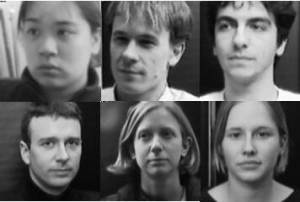
\includegraphics{training-images.jpg}
\begin{figure}[h]
 \begin{center}
 \centering
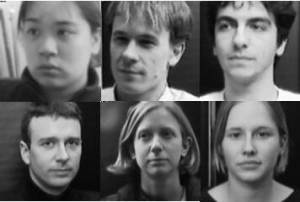
\includegraphics[scale=0.5]{training-images.jpg} \caption{Sample Faces. }
 \end{center}\end{figure}
\item Represent each image $I_i$ as a vector $\Gamma_i$.
\begin{equation}
\label{arrequation}
I_i  = \left[ {\begin{array}{*{20}c} {a_{11} } & {a_{12} } &\ldots& {a_{1N} }  \\
   {a_{21} } & {a_{22} } &  \ldots   & {a_{2N} }  \\
    \vdots  &  \vdots  &  \ddots   & {}  \\
   {a_{N1} } & {a_{N2} }  & {} & {a_{NN} }  \\
\end{array}} \right]_{NxN} \Rightarrow\left[
{\begin{array}{*{20}c}
   {a_{11} }  \\
   {\vdots}  \\
    {a_{1N} }  \\
     {a_{21}}  \\
        {\vdots}  \\
   {a_{2N} }  \\
   {\vdots}  \\
   {a_{NN} }  \\
\end{array}} \right]_{N^2 x1} = \Gamma _i
\end{equation}
\item Find the average or the mean face vector  $\Psi$

\begin{equation}
\Psi  = \frac{1}{M}\sum\limits_{i = 1}^M {\Gamma _i }
\end{equation}
\item  Subtract the mean face $\Psi$ from each face vector $\Gamma_i$ to get a set of vectors $\Phi_i$. The purpose of subtracting the mean image from each image vector is to be left with only the distinguishing features from each face and (removing)  in a way information that is common.
\begin{equation}
\Phi _i  = \Gamma_i  - \Psi
\end{equation}
\item  Find the Covariance matrix $C$:
\begin{equation}
C = AA^T
\end{equation} , where $A = \left[ {\begin{array}{*{20}c}
   {\Phi _1 } & {\Phi_2} & {\dots} & {\Phi _M }  \\
\end{array}} \right]
$
Note that the Covariance matrix has simply been made by putting one modified image vector obtained in  one column each.

Also note that $C$is a $N^2xN^2$ matrix and $A$ is a $NxM$ matrix.


\item  Instead of the Matrix $AA^T$  consider the matrix $A^TA$ .


\item Find the $M$ best  Eigenvectors of $C=A^TA$. using the relation of $u_i=Av_i$  Also keep in mind that $\left\| {u_i} \right\| = 1.$ where  $u_i$ is the eigen vector of $C$ and $v_i$ is the eigen value of the matrix $C$.



\item Select the best  Eigenvectors, the selection of these Eigenvectors is done heuristically.




\item Finding Weights:\\

The Eigenvectors found at the end of the previous section,  when converted to a matrix in a process that is reverse to that in STEP \ref{facereg}, have a face like appearance. Since these are Eigenvectors and have a face like appearance, they are called Eigenfaces. Sometimes, they are also called as Ghost Images because of their weird appearance.

Now each face in the training set (minus the mean),$\Phi_i$  can be represented as a linear combination of these Eigenvectors   $u_j$:
  \begin{equation}
\Phi_i  = \sum\nolimits_{j = 1}^k {\omega_j u_j}
  \end{equation}
, where  $u_j$�s are Eigenfaces and $\omega_j$ are the weights and can be calculated as :
\begin{equation}
\label{weighteq}
\omega _j  = u_j^T \Phi _i
\end{equation}
Each normalized training image is represented in this basis as a vector $\Omega$.
\end{enumerate}
\subsection{PSO clustering}

On the Merwe and Engelbrechet \cite{psoclustering} Method. The particle $X_i$ is constructed that
\begin{equation}
X_i=\left( m_{i1}, m_{i2}, m_{i3},\dots, m_{iN_c}\right)
\end{equation}
where $N_c$ is the number of clusters to be formed and $m_{ij}$ corresponds to the $j^{th}$ centroid of the  $i^{th}$ particle, the centroid of the cluster $C_{ij}$. Thus single particle represents a candidate solution to a given clustering algorithm. Each particle is evaluated using the following equation:
% \begin{equation}
% F_c=\frac{\sum^{N_c}_{j=1}\right[\sum_{\forall Z_j \epsilon C_{ij}}\frac{ d\right(Z_p,m_{ij}\left)}{|C_{ij}|}  \left]}{N_c}
% \end{equation}
\begin{equation}
F_c  = \frac{{\sum\nolimits_{j = 1}^{N_c } {\left[ {\sum\limits_{\forall z_j  \in C_{ij} } {\frac{{d(z_p ,m_{ij} )}}{{\left| {C_{ij} } \right|}}} } \right]} }}{{N_c }}
\end{equation}
where $F_c$ is the fitness function, $N_c$ is the number of clusters in the particle, $Z_p$ denotes the $p^{th}$ data vector $\left| {C_{ij} } \right|$ is the number of data vectors belonging to the cluster $C_{ij}$ and $d$ is the Euclidian distance between $Z_p$ and $m_{ij}$.


The clustering algorithm prposed by Merwe and Engelbrecht \cite{} can be as follows:
% \begin{algorithm}
%  \caption{ Discrete Particle Swarm Algorithm }
%  \label{DPSOalg}
\begin{algorithmic}
%\begin{verbatim}

\STATE  Generate $N$ particles with $N_c$ clusters  ($P_i,$ $\dots,$ $P_{N_c}$)
\STATE Initialize the clusters centroids for each particle randomly
\FOR{i=0 \TO $t_{max}$}
  \FOR{ each particle  $p_i$}
    \FOR{ each data vector  $zp$}
        \STATE   Calculate distance $d(zp,m_{ij})$ from cluster centroid.
        \STATE   Assign $zp$ to cluster $C_{ij}$ such that
        \STATE   $d(zp,m_{ij})=min \forall k=1,\dots,N_c {d(zp,m_{ik})}$
    \ENDFOR
    \STATE  Compute the Fitness function for the particle.
     \STATE  Update the global best and local best
     \STATE  Move all particle using PSO equations.
     \ENDFOR
  \ENDFOR
 \RETURN global best
%\end{verbatim}

 \end{algorithmic}
\section{System}


\begin{figure}[h]
 \begin{center}
 \centering
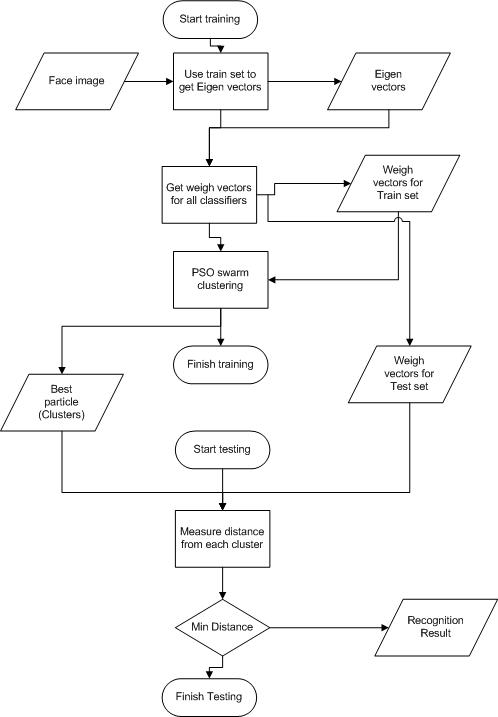
\includegraphics[scale=0.5]{blockchart.jpg} \caption{ The flow Chart}
 \end{center}\end{figure}

Both previous algorithms  were implemented and tested for correctness. Also the k-means algorithm was used to compare the result of the PSO clustering algorithm. The code was implemented using Matlab and using a Database as train and test set. The Databases contains 50 persons and 4 images per person. Currenlty all the images are used for training and the same set is used for testing.


The PSO algorithm is used to clusters each face weights computed using equation \ref{weighteq}. The algorithms first compute the eigen vectors for all 50 faces as explained in section \ref{facereg}. The computed $u_j$ is used to compute the weights for each image in the database is computed which generate a data matrix of 150 X 50 ( number of image X weight vector (no of eigenfaces)). The clustering algorithm is used to get center weigh vector for each person. I choose the number of clusters same as number of person for easier recognition step.


The recognition step will be easier as to compute the weigh vector of the input image and then compute the distance from each cluster centroid. The cluster with the min distance is the cluster of the face.
\subsection{Nelder Enhancment}

\section{Results}
Two different databases was processed, the first contains 60 indian faces with 11 different samples with different poses and experisions. The second database is 120 eroupian faces each has 20 samples. The database is processed to the input format for the particle algorithm. The data is then divided into training and testset. The percentage can be changed and changed to cross validate the results and experiments.

\subsection{Experiments Finding PSO paramters}
\begin{table}
	\centering
		\caption{PSO Result }
	\label{tab:PSO1}
	%\scalebox{0.99}{
		\begin{tabular}{|l|c|c|c|c|c|}
		 \hline
C1 &	1	&1.2&	1.6&	1.8 &	2	\\ \hline
	&70.893	&70.893	&70.605	&70.029	&69.741 \\  \hline
C2	&	1	&1.2&	1.6&	1.8 &	2	\\ \hline
	&70.89	&70.61	&70.89	&69.45	&69.45 \\ \hline
W	&0.5&	1	&1.5	&2&	4	\\ \hline
	&69.74	&70.89&	70.89	&70.32&	70.89	\\ \hline
\end{tabular}
		%}
\end{table}


\subsection {Comparing With other systems}

\subsection{ Comparing Nelder enhancement}

\section{Conclusion}
\section{future work}
% \subsection{Subtitle}
%
% Plain text.
%
% \subsection{Another subtitle}
%
% More plain text.
\bibliographystyle{model1a-num-names}
\bibliography{mybibfile,library}

\end{document}
